\documentclass[preprint,12pt, a4paper]{elsarticle}

\usepackage{amssymb}
\usepackage{lineno}
\usepackage{float}
\usepackage{hyperref}
\usepackage{listings}
\lstset{language=Python}

\restylefloat{table}

\journal{SoftwareX}

\begin{document}

\begin{frontmatter}

	\title{cluster-over-sampling: A package for clustering-based oversampling}

	\author{Georgios Douzas\corref{nova}}
	\ead{gdouzas@novaims.unl.pt}

	\author{Fernando Bacao}
	\ead{bacao@novaims.unl.pt}

	\address{NOVA Information Management School, Universidade Nova de Lisboa}

	\cortext[nova]{Postal Address: NOVA Information Management School, Campus de Campolide, 1070-312 Lisboa, Portugal, Telephone: +351 21 382 8610}

	\begin{abstract}
	Learning from imbalanced data is a common and challenging problem in supervised learning. Standard classifiers are designed to handle balanced class distributions. While different strategies exist to tackle this problem, methods that generate artificial data to achieve a balanced class distribution, called oversampling algorithms, are more versatile than modifications to the classification algorithms. SMOTE algorithm, the most popular oversampler, as well as any other oversampling method based on it, generates synthetic samples along line segments that join minority class instances. SMOTE addresses only the issue of between-classes imbalance. On the other hand, by clustering the input space and applying any oversampling algorithm for each resulting cluster with appropriate resampling ratio, the within-classes imbalanced issue can be addressed. This approach, implemented in the \texttt{cluster-over-sampling} Python open source project, has been shown in multiple publications, using a variety of datasets, to outperform other standard oversamplers. In this paper we describe \texttt{cluster-over-sampling} in detail and make it available to the machine learning community. An important point is that the implementation integrates effortlessly with the Scikit-Learn ecosystem. Therefore, machine learning researchers and practitioners can integrate it directly to any pre-existing work.
	\end{abstract}

	\begin{keyword}
		Machine learning \sep Classification \sep Imbalanced learning \sep Oversampling \sep Clustering
	\end{keyword}

\end{frontmatter}

\begin{table}[H]
	\begin{tabular}{|p{6.5cm}|p{6.5cm}|}
		\hline
		Code metadata                                                    &                                                                                       \\
		\hline
		Current code version                                             & v0.1.1                                                                                \\
		\hline
		Permanent link to code/repository used for this code version     & \url{https://github.com/AlgoWit/cluster-over-sampling}                                \\
		\hline
		Legal Code License                                               & MIT                                                                                   \\
		\hline
		Code versioning system used                                      & git                                                                                   \\
		\hline
		Software code languages, tools, and services used                & Python, Travis CI, AppVeyor, Read the Docs, Codecov, CircleCI, zenodo, Anaconda Cloud \\
		\hline
		Compilation requirements, operating environments \& dependencies & Linux, Mac OS, Windows                                                                \\
		\hline
		If available Link to developer documentation/manual              & \url{https://cluster-over-sampling.readthedocs.io/}                                   \\
		\hline
		Support email for questions                                      & \href{mailto:georgios.douzas@gmail.com}{georgios.douzas@gmail.com}                    \\
		\hline
	\end{tabular}
	\caption{Code metadata}
	\label{}
\end{table}

\linenumbers

%% main text

\section{Motivation and significance}
\label{motivation}

\subsection{Introduction}
\label{introduction}

The imbalanced learning problem describes the case where in a machine learning classification task, using datasets with binary or multi-class targets, one of the classes, called the majority class, has a significantly higher number of samples compared to the remaining classes, called the minority class(es) \cite{Chawla2003}. Learning from imbalanced data is a non-trivial problem for both academic researchers and industry practitioners that can be frequently found in multiple domains such as chemical and biochemical engineering, financial management, information technology, security, business, agriculture or emergency management \cite{Haixiang2017}.

A bias towards the majority class is induced when imbalanced data are used to train standard machine learning algorithms. This results in low classification accuracy, especially for the minority class(es), when the classifier is evaluated on unseen data. An important measure for the degree of data imbalance is the Imbalance Ratio ($IR$), defined as the ratio between the number of samples of the majority class and each of the minority classes. Using a rare disease detection task as an example, with 1\% of positive cases corresponding to an $IR=\frac{0.99}{0.01}=99$, a trivial classifier that always labels a person as healthy will score a classification accuracy of 99\%. However in this case, all positive cases remain undetected. The observed values of $IR$ are often between 100 and 100.000 \cite{Chawla2002}, \cite{Barua2014}. Figure \ref{fig:imbalanced} presents an example of imbalanced data in two dimensions as well as the decision boundary identified by a typical classifier when they are used as a training set.

\begin{figure}[H]
	\centering
	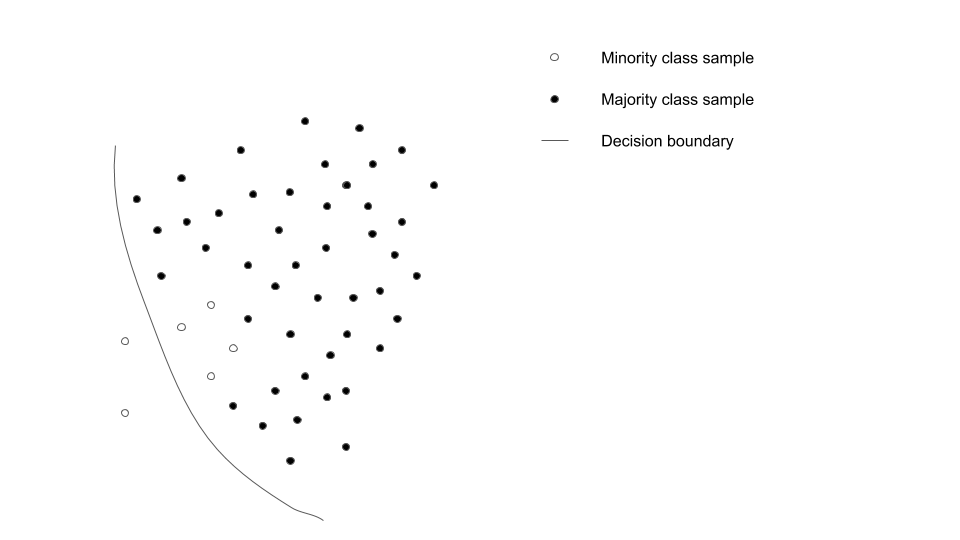
\includegraphics[width=14cm, keepaspectratio]{../analysis/imbalanced_problem}
	\caption{Imbalanced data in two dimensions. The decision boundary of a typical classifier shows a bias towards the majority class.}
	\label{fig:imbalanced}
\end{figure}

\subsection{Oversampling algorithms}
\label{oversampling}

Various approaches have been proposed to improve classification results when the training data are imbalanced, a case also known as between-class imbalance. The most general approach, called oversampling, is the generation of artificial data for the minority class(es) \cite{Fernandez2013}. Synthetic Minority Oversampling Technique (SMOTE) \cite{Chawla2002} was the first non-trivial oversampler proposed and remains the most popular one. Although SMOTE has been shown to be effective for generating artificial data, it also has some drawbacks \cite{He2009}. In order to improve the quality of the artificial data many variants of SMOTE have been proposed. Nevertheless, they utilize the SMOTE data generation mechanism, which consists of a linear interpolation between minority class samples to generate synthetic instances as shown in figure \ref{fig:smote}.

\begin{figure}[H]
	\centering
	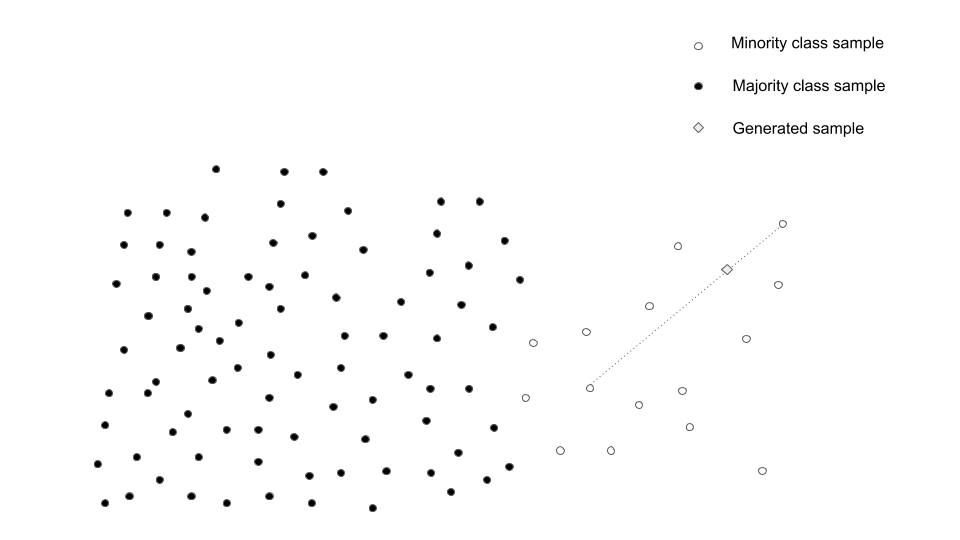
\includegraphics[width=1\linewidth]{../analysis/smote}
	\caption{Visual representation of the SMOTE data generation mechanism.}
	\label{fig:smote}
\end{figure}

A Python implementation of SMOTE and several of its variants is available in the \href{https://imbalanced-learn.org/stable/}{Imbalanced-Learn} \cite{Lemaitre2016} library, which is fully compatible with the popular machine learning toolbox \href{https://scikit-learn.org/stable/}{Scikit-Learn} \cite{Pedregosa2011}.

\subsection{Clustering-based oversampling}
\label{clustering-based-oversampling}

In addition to between-class imbalance, within-class imbalance refers to the case where areas of sparse and dense minority class instances exist. As the first step of generating synthetic samples, the SMOTE data generation mechanism selects randomly, with uniform probability, minority class instances. Consequently, dense minority class areas have a high probability of being inflated further, while the sparsely populated are likely to remain sparse. This allows to combat between-class imbalance, while the issue of within-class imbalance is ignored \cite{Prati2004}.

On the other hand, clustering-based oversampling, as presented in \cite{Douzas2017a} and \cite{Douzas2018}, aims to deal with both between-class and within-class imbalance problems. Initially a clustering algorithm is applied to the input space. The resulting clusters allow to identify sparse and dense minority class(es) areas. A small IR, relatively to a threshold, of a particular cluster is used as an indicator that it can be safely used as a data generation area, i.e. noise generation is avoided. Furthermore, sparse minority clusters are assigned more synthetic samples, which alleviates within-class imbalance.

Specific realizations of the above approach are SOMO \cite{Douzas2017a} and KMeans-SMOTE \cite{Douzas2018} algorithms. Empirical studies have shown that both algorithms outperform SMOTE and its variants across multiple imbalanced datasets, classifiers and evaluation metrics. In this paper, we present a generic Python implementation of clustering-based oversampling, in the sense that any combination of a Scikit-Learn compatible clusterer and Imbalanced-Learn combatible oversampler can be selected to produce an algorithm that identifies clusters on the input space and applies oversampling on each one of them.  In section \ref{software-description}, the software description is given while section \ref{examples} provides a demonstrative example of its functionalities.

\section{Software description}
\label{software-description}

The \texttt{cluster-over-sampling} software project is written in Python 3.7. It contains an object-oriented implementation of the clustering-based oversampling procedure as well as detailed \href{https://cluster-over-sampling.readthedocs.io/}{online documentation}. The implementation provides an API that is compatible with Imbalanced-Learn and Scikit-Learn libraries. Therefore, standard machine learning functionalities are supported while the generated clustering-based oversampling algorithm, composed by a clusterer and an oversampler, contains the initial oversampler functionality as a special case.

\subsection{Software architecture}
\label{architecture}

The \texttt{cluster-over-sampling} project contains the Python package \texttt{clover}. The main modules of \texttt{clover} are called \texttt{distribution} and \texttt{over\_sampling}. The \texttt{distribution} module implements the functionality related to the distribution of the generated samples to the identified clusters, while \texttt{over\_sampling} implements the functionality related to the generation of artificial samples. Both of them are presented in detail below.

\subsubsection{Module \texttt{distribution}}
\label{distribution}

The module \texttt{distribution} contains the files \texttt{base.py} and \texttt{density.py}. The former provides the implementation of the \texttt{BaseDistributor} class, the base class for distributors, while the later includes the \texttt{DensityDistributor} class, a generalization of the density based distributor presented in \cite{Douzas2017a} and \cite{Douzas2018}, that inherits from \texttt{BaseDistributor}. Following the Scikit-Learn API, \texttt{BaseDistributor} includes the public methods \texttt{fit} and \texttt{fit\_distribute}. The \texttt{fit\_distribute} method calls the \texttt{fit} method and returns two Python dictionaries that describe the distribution of generated samples inside each cluster and between clusters, respectively. Specifically, the \texttt{fit} method calculates various statistics related to the distribution process, while it calls \texttt{\_fit} method to calculate the actual intra-cluster and inter-cluster distributions. This is achieved by invoking the \texttt{\_intra\_distribute} and \texttt{\_inter\_distribute} methods. The \texttt{BaseDistributor} class provides a trivial implementation of them, that should be overwritten when a realization of a distributor class is considered. Consequently, \texttt{DensityDistributor} overwrites both methods as well as the \texttt{\_fit} method. The later calls the methods \texttt{\_identify\_filtered\_clusters} and \texttt{\_calculate\_clusters\_density} that identify the clusters used for data generation and calculate their density, respectively. Subsection \ref{functionality} provides a detailed description of the initialization and functionality of the \texttt{DensityDistributor} class. Figure \ref{fig:distributor_class_diagram} shows a visual representation of the above classes and functions hierarchy.

\begin{figure}[H]
	\centering
	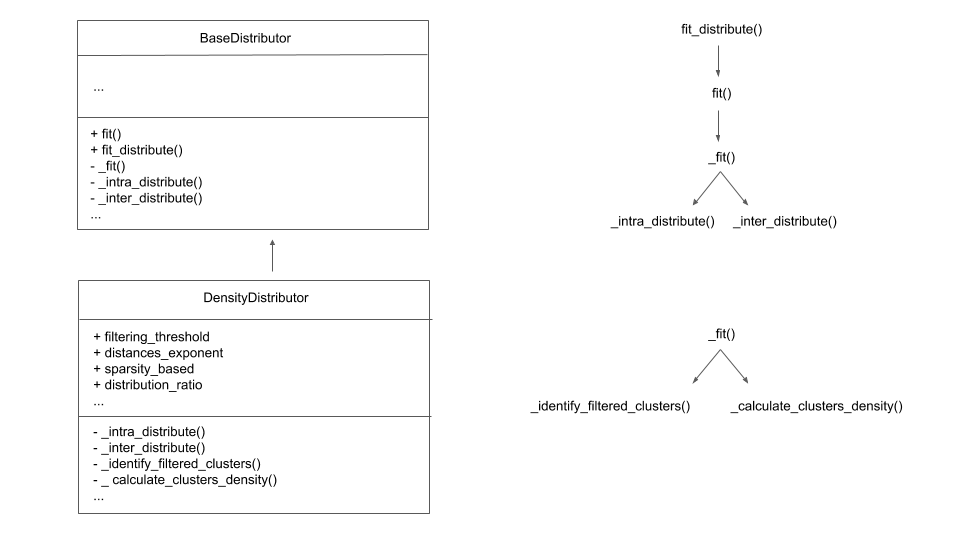
\includegraphics[width=1\linewidth]{../analysis/distributor_class_diagram}
	\caption{UML BaseDistributor and DensityDistributor class diagrams and callgraphs of main classes and methods.}
	\label{fig:distributor_class_diagram}
\end{figure}

\subsubsection{Module \texttt{oversampling}}
\label{oversampling}

The module \texttt{over\_sampling} contains the files \texttt{base.py} and \texttt{monkey\_patching.py}. The former provides the implementation of the \texttt{BaseClusterOverSampler} class, an extension of the Imbalanced-Learn's \texttt{BaseOverSampler} class, while the later enhances the main oversamplers provided by Imbalanced-Learn with the functionality required by clustering-based oversampling. The initializer of \texttt{BaseClusterOverSampler}, compared to \texttt{BaseOverSampler}, includes the extra parameters \texttt{clusterer} and \texttt{distributor}. Also following the Imbalanced-Learn API, \texttt{BaseClusterOverSampler} includes the public methods \texttt{fit} and \texttt{fit\_resample}. It also inherits from \texttt{BaseOverSampler}, the base class of oversamplers that is implemented in Imbalanced-Learn. The \texttt{fit} method calculates various statistics related to the resampling process, while the \texttt{fit\_resample} method returns an enhanced version of the input data by appending the artificially generated samples. Specifically, \texttt{fit\_resample} calls the \texttt{\_fit\_resample} method that in turn calls the \texttt{\_intra\_sample} and \texttt{\_inter\_sample} methods to generate the intra-cluster and inter-cluster artificial samples, respectively. This is achieved by invoking the \texttt{\_fit\_resample\_cluster} method that implements the data generation mechanism. Therefore every oversampler that inherits from the \texttt{BaseClusterOverSampler} class should overwrite \texttt{\_fit\_resample\_cluster}, providing a concrete implementation of the oversampling process. This has been done for the main oversamplers of Imbalanced-Learn through the \texttt{monkey\_patching} module. Specifically, for each oversampler the \texttt{\_fit\_resample\_cluster} method has been set equal to the \texttt{\_fit\_resample} method. Subsection \ref{functionality} provides a detailed description of the initialization and functionality of the various oversamplers, enhanced by the clustering process. Figure \ref{fig:oversampler_class_diagram} shows a visual representation of the above classes and functions hierarchy.

\begin{figure}[H]
	\centering
	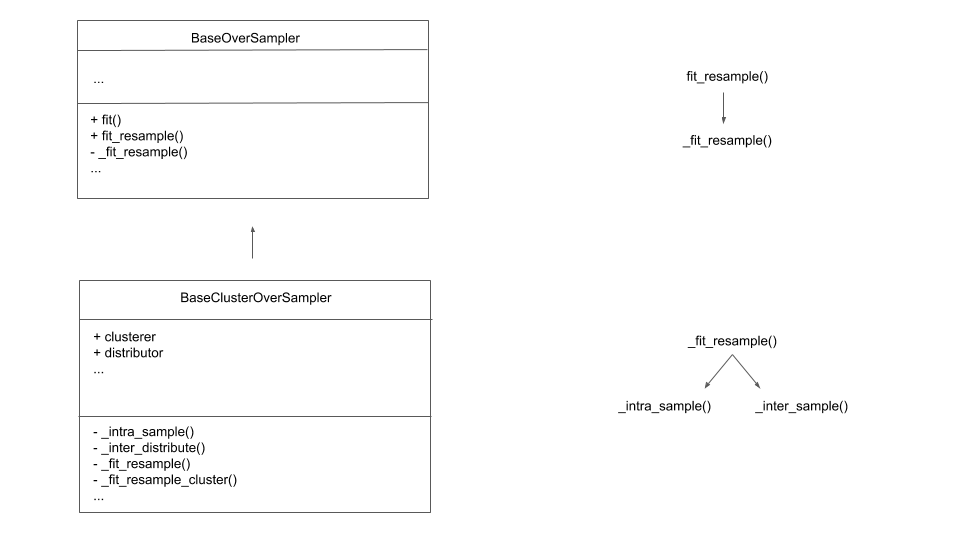
\includegraphics[width=1\linewidth]{../analysis/oversampler_class_diagram}
	\caption{UML BaseOverSampler and BaseClusterOversampler class diagrams and callgraphs of main classes and methods.}
	\label{fig:oversampler_class_diagram}
\end{figure}

\subsection{Software Functionalities}
\label{functionality}

As it was mentioned in subsection \ref{oversampling}, \texttt{cluster-over-sampling} extends Imbalanced-Learn's functionality by clustering the input space before oversampling is applied. This is achieved through the implementation of the \texttt{BaseClusterOverSampler} class, an extension of Imbalanced-Learn's \texttt{BaseOverSampler} class. Oversamplers that inherit from \texttt{BaseClusterOverSampler}, compared to oversamplers inheriting from \texttt{BaseOverSampler}, require two additional initialization parameters: \texttt{clusterer} and \texttt{distributor}. Their default values are for both parameters equal to \texttt{None}, a case that corresponds to the usual oversampling procedure i.e. no clustering applied to the input space. On the other hand if the parameter \texttt{clusterer} is equal to any Scikit-Learn compatible clustering algorithm then clustering of the input space is initially applied, followed by oversampling in each cluster with the distribution of generated samples given by the \texttt{distributor} parameter. The default \texttt{distributor} value is an instance of \texttt{DensityDistributor} class as described in subsection \ref{distribution}. The initializer of \texttt{DensityDistributor} includes the following parameters: \texttt{filtering\_threshold}, \texttt{distances\_exponent}, \texttt{sparsity\_based} and \texttt{distribution\_factor}. The first parameter is used to identify the filtered clusters, i.e. clusters of samples that are included in the data generation process. The second parameter modifies the density calculation of the filtered clusters by increasing the effect of euclidean distances between samples. The third parameter selects whether generated samples are assigned to filtered clusters inversly proportonial to their density. Finally the last parameter adjusts the intra-cluster to inter-cluster proportion of generated samples, while it applies only to clusterers that support a neighborhood structure. Once the \texttt{DensityDistributor} object is initialized with a specific parametrization, it can be used to distribute the generated samples to the clusters identified by any clustering algorithm.

Resampling is achieved by using the two main methods of \texttt{fit} and \texttt{fit\_resample} of any oversampler inheriting from \texttt{BaseClusterOverSampler}. More specifically, both of them take as input parameters the input matrix \texttt{X} and target labels \texttt{y}. Following the Scikit-Learn API, both \texttt{X}, \texttt{y} are array-like objects of appropriate shape. The first method computes various statistics which are used to resample \texttt{X}, while the second method does the same but additionally returns a resampled version of \texttt{X} and \texttt{y}.

The \texttt{cluster-over-sampling} project has been designed to integrate with the Imbalanced-Learn toolbox and the Scikit-Learn ecosystem. Therefore any oversampler that inherits from \texttt{BaseClusterOverSampler} can be used in a machine learning pipeline, through Imbalanced-Learn's class \texttt{Pipeline}, that automatically combines \texttt{samplers}, \texttt{transformers} and \texttt{estimators}. The next section provides examples of the above functionalities.

\section{Illustrative examples}
\label{examples}

\subsection{Basic example}

An example of resampling an imbalanced dataset using the \texttt{fit\_resample} method is presented in Listing \ref{lst:basic}. Initially, a binary-class imbalanced dataset is generated. Next, a \texttt{SMOTE} oversampler is initialized using \texttt{KMeans} as a clusterer. This effectively corresponds to the KMeans-SMOTE algorithm as presented in \cite{Douzas2018}. Finally, the oversampler's \texttt{fit\_resample} method is used to resample the data. Printing the class distribution before and after resampling confirms that the resampled data \texttt{X\_res}, \texttt{y\_res} are perfectly balanced. \texttt{X\_res}, \texttt{y\_res} can be used as training data for any classifier in the place of \texttt{X}, \texttt{y}.

\begin{lstlisting}[caption={Resampling of imbalanced data using the \texttt{fit\_resample} method of KMeans-SMOTE oversampling algorithm.},label={lst:basic}]
# Import classes and functions.
from collections import Counter
from clover.over_sampling import SMOTE
from sklearn.cluster import KMeans
from sklearn.datasets import make_classification

# Generate an imbalanced a binary class dataset.
X, y = make_classification(
    random_state=23, 
	n_classes=2,
	n_features=5,
    n_samples=1000,
    weights=[0.8, 0.2]
)

# Create KMeans-SMOTE object with default hyperparameters.
kmeans_smote = SMOTE(clusterer=KMeans(random_state=4), random_state=10)

# Resample the imbalanced dataset.
X_res, y_res = kmeans_smote.fit_resample(X, y) 

# Print number of samples per class for initial and resampled data. 
init_count = list(Counter(y).values())
resampled_count = list(Counter(y_res).values())

print(f'Initial class distribution: {init_count}.') 
# Initial class distribution: [792, 208].

print(f'Resampled class distribution: {resampled_count}.')
# Resampled class distribution: [792, 792].
\end{lstlisting}

\subsection{Machine learning pipeline}

As mentioned before, any clustering-based oversampler can be used as a part of a machine learning pipeline. Listing \ref{lst:pipeline} presents a pipeline composed by the combination of Borderline SMOTE oversampler and hierarchical clustering, a PCA tranformation and a decision tree classifier. The pipeline is trained on multi-class imbalanced data and evaluated on a hold-out set. The user applies the process in a simple way while the internal details of the calculations are hidden.

\begin{lstlisting}[caption={Training and evaluation of a machine learning pipeline that contains the AgglomerativeClustering-BorderlineSMOTE algorithm.},label={lst:pipeline}]
# Import classes and functions.
from clover.over_sampling import BorderlineSMOTE
from sklearn.datasets import make_classification
from sklearn.decomposition import PCA
from sklearn.tree import DecisionTreeClassifier
from sklearn.model_selection import train_test_split
from sklearn.metrics import f1_score
from sklearn.cluster import AgglomerativeClustering
from imblearn.pipeline import make_pipeline

# Generate an imbalanced multi-class dataset.
X, y = make_classification(
	random_state=23, 
	n_classes=3, 
	n_informative=10,
	n_samples=500,
	weights=[0.8, 0.1, 0.1]
)

# Split the data to training and hold-out sets.
X_train, X_test, y_train, y_test = train_test_split(X, y, random_state=10)

# Create the pipeline's objects with default hyperparameters.
hclusterer_bsmote = BorderlineSMOTE(clusterer=AgglomerativeClustering(), random_state=19)
pca = PCA()
clf = DecisionTreeClassifier(random_state=3)

# Create the pipeline.
pip = make_pipeline(hclusterer_bsmote, pca, clf)

# Fit the pipeline to the training set.
pip.fit(X_train, y_train)

# Evaluate the pipeline on the hold-out set using the F-score.
test_score = f1_score(y_test, pip.predict(X_test), average='micro')

print(f'F-score on hold-out set: {test_score:.2f}.')
# F-score on hold-out set: 0.78.
\end{lstlisting}

\section{Impact and conclusions}

Classification of imbalanced datasets is a challenging task for standard machine learning algorithms. In addition to between-class imbalance, within-class imbalance refers to the case where areas of sparse and dense minority class instances exist. Clustering-based oversampling, aims to deal with both between-class and within-class imbalance problems.

The \texttt{cluster-over-sampling} project provides the only Python implementation, to the best of our knowledge, that provides a generic way to construct any clustering-based oversampler. A significant advantage of this implementation is that it is built on top of the Scikit-Learn's ecosystem and therefore it can be easily used in typical machine learning workflows. Also, the public API of any clustering-based oversampler is an extension of the one provided in Imbalanced-Learn. This means that users of Imbalanced-Learn and Scikit-Learn, that apply oversampling on imbalanced data, can integrate the \texttt{cluster-based-oversampler} package in their existing work in a straightforward manner.

\section{Conflict of interest}

We wish to confirm that there are no known conflicts of interest associated with this publication and there has been no significant financial support for this work that could have influenced its outcome.

\bibliography{references}
\bibliographystyle{elsarticle-num}
\end{document}
\endinput

